%!TEX root = ../thesis-main.tex

\chapter{Introduzione}\label{chap:introduction}
Il mondo del software ha scritto diverse decadi di storia. Sin dagli anni '50, quando i primi calcolatori programmabili hanno fatto il loro ingresso sul mercato, il software ha assunto un ruolo sempre più pervasivo nella vita quotidiana delle persone. Oltre ad essere parte integrante dei sistemi informativi delle aziende, lo possiamo trovare anche all'interno di automobili, elettrodomestici e tantissimi strumenti con la quale abbiamo a che fare nella nostra quotidianità. La crescente diffusione del software ha introdotto la necessità di progettare metodologie di sviluppo solide e versatili. Uno dei primi è il \textbf{modello a cascata} il quale struttura il processo di realizzazione del software in fasi sequenziali lineari. Il modello riprende la tipica organizzazione della produzione manifatturiera e fu progressivamente abbandonato con l'evolversi delle richieste del mercato. Successivamente prese piede il concetto di modelli iterativi come il \textbf{modello a spirale} in cui il processo di sviluppo è suddiviso in fasi multiple ripetute più volte (iterazioni). Gli ultimi decenni hanno dato vita a un nuovo modello, considerato lo standard dell'industria, la \textbf{metodologia agile}. Quest'ultima non rappresenta un unico modello, ma un insieme di modelli iterativi costruiti sulla base dei principi definiti all'interno del manifesto agile. Questi mettono in primo piano un ambiente autonomo e dinamico in cui sono fondamentali: cicli di sviluppo brevi, continui miglioramenti, la comunicazione col cliente e la consegna tempestiva di funzionalità. Il progetto esposto in questo documento introduce un evoluzione del concetto agile nato recentemente nel mondo dello sviluppo del software, conosciuto come ``DevOps".

\section{Contesto}
Con l'avvento di internet il concetto di software come un entità sviluppata e finita ha completamente cessato di esistere. Mediante la rete è diventato semplice ed efficiente distribuire un programma e fornire un ulteriore supporto attraverso aggiornamenti evolutivi e correttivi. Il fenomeno è cresciuto tanto da aver dato luce alla pratica del rilascio di applicazioni deliberatamente non complete, le quali attraverso il feedback degli utenti evolvono verso un prodotto finito. Il manifesto agile ha introdotto la cultura di emettere frequenti rilasci di nuove versioni del software, rendendo la distribuzione un punto cardine all'interno del ciclo di vita di esso. Dietro lo sviluppo rapido di nuove funzionalità è necessario il rilascio di queste altrettanto velocemente, la filosofia DevOps nasce per soddisfare questa esigenza.

\subsection{DevOps}
La metodologia DevOps (termine nato dalla contrazione di ``Development" ed ``Operations") si è formata intorno al 2008 con l'idea chiave di unire il team di sviluppo ed il team operativo. Il principale catalizzatore di questo concetto è stata la necessità di affrontare inefficienze nelle fasi del ciclo di vita del software. Differentemente dalla metodologia agile, DevOps è una filosofia di sviluppo software che esprime attraverso tre pilastri il suo obiettivo:

\begin{itemize}
	\item il \textbf{flusso}, il miglioramento del flusso di lavoro lungo l'intero processo di produzione, ciò significa ottimizzare il processo dall'idea, fino alla generazione di valore con il software in produzione.
	\item Il \textbf{feedback}, mediante cicli di feedback rapidi si garantisce la scoperta di difetti nel codice nelle fasi iniziali del ciclo di vita del prodotto. Ciò comporta rapide correzioni, minor debito tecnico e la garanzia di possedere in qualsiasi momento un software stabile e qualitativamente pronto ad un rilascio.
	\item L'\textbf{apprendimento continuo}, la filosofia DevOps promuove la sperimentazione continua: interrogarsi regolarmente sui possibili miglioramenti attuabili assumendosi i rischi che il processo può recare.
\end{itemize}

Le nozioni fornite dalla cultura DevOps ricoprono diversi ambiti e non si limitano agli aspetti tecnici del ciclo di vita del software. Nella pratica esistono diverse tecnologie che concorrono allo sviluppo di processi conformi alla metodologia presentata.

\begin{figure}[htb]
	\centering
	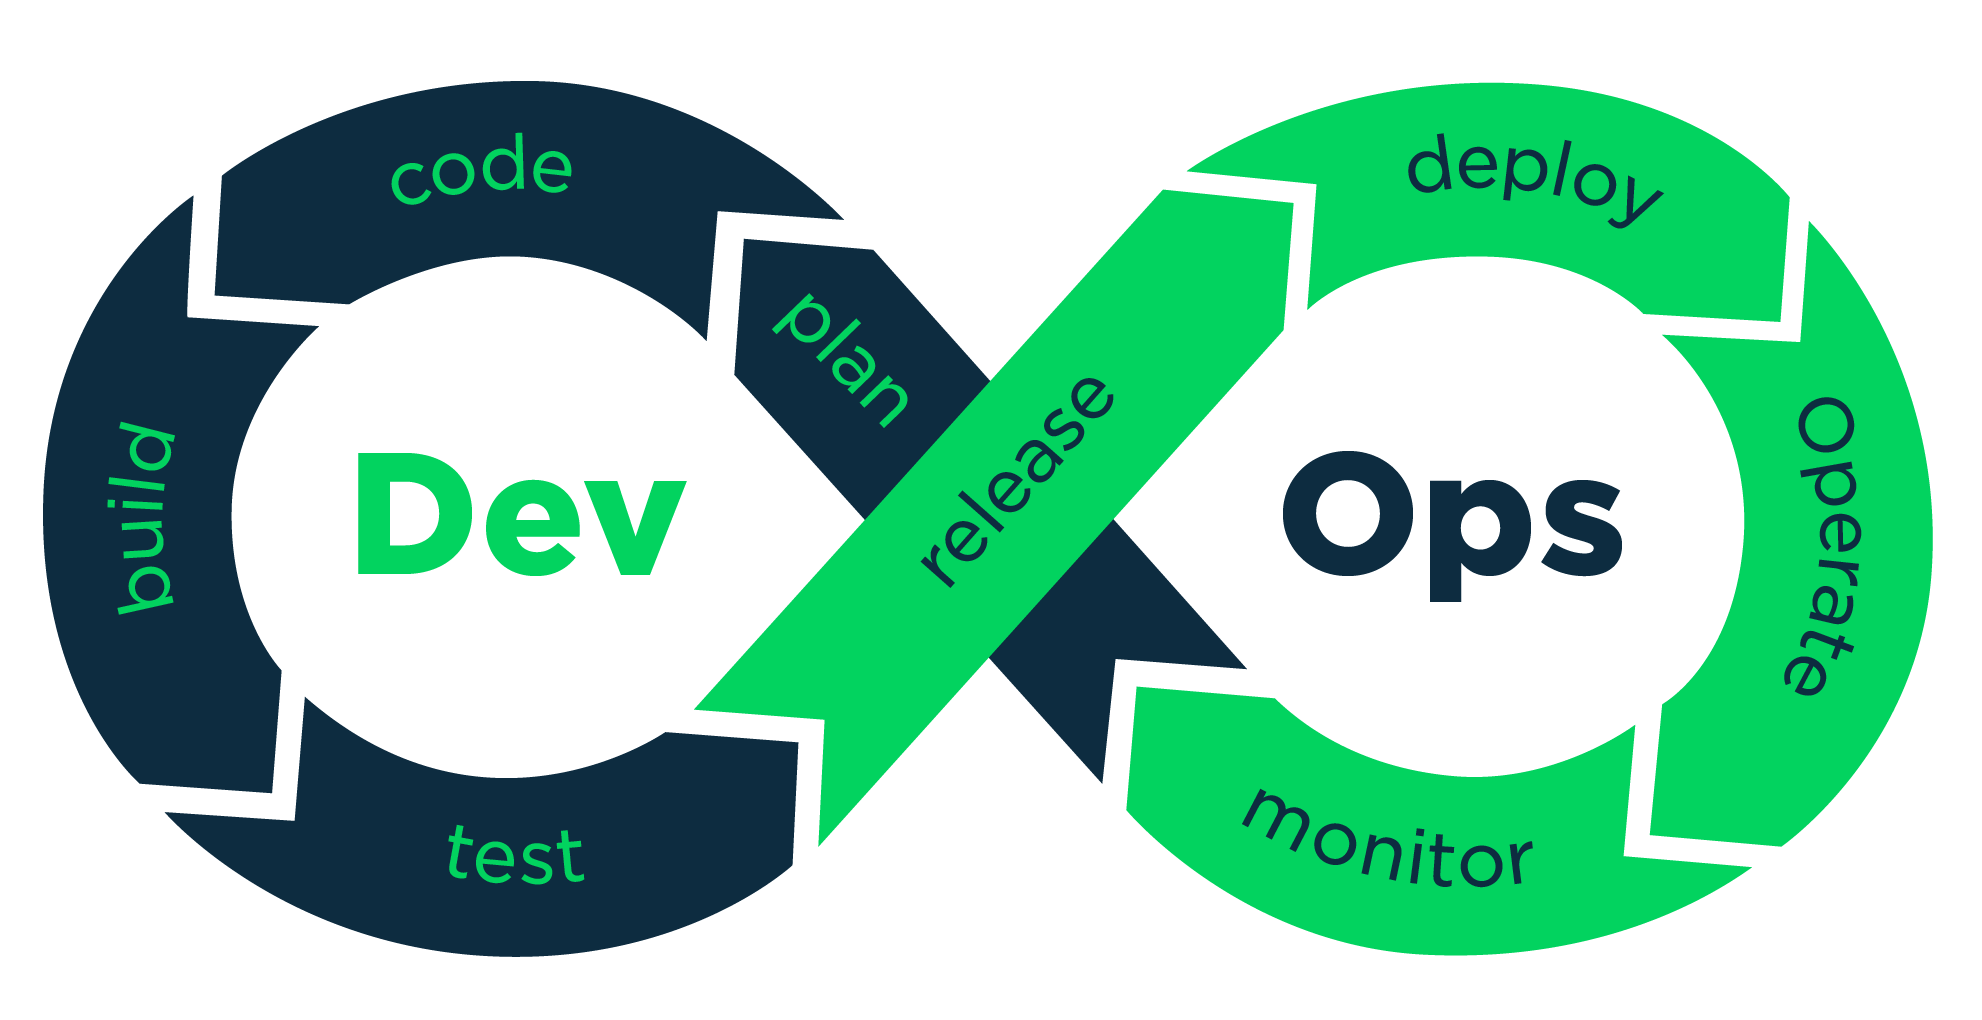
\includegraphics[width=.8\linewidth]{figures/devops-process.png}
	\caption{Le fasi della metodologia DevOps}
	\label{fig:devops-process}
\end{figure}

Il modello illustrato nella figura \ref{fig:devops-process} rappresenta la visione del ciclo di vita del software per la filosofia DevOps. La posizione delle fasi così configurata in modo da rappresentare il simbolo dell'infinito è utilizzata per simboleggiare il concetto di continuità che la metodologia utilizza. Essa è introdotta all'interno del flusso mediante un altro pilastro: l'\textit{automazione}. Grazie all'automazione, gli sviluppatori possono delegare compiti complessi o ripetitivi a sistemi esterni configurando tre componenti chiave: un evento, un'azione e il risultato atteso. Quando si verifica un evento specifico, un'entità esterna esegue un insieme di azioni predeterminate, il cui successo o fallimento viene determinato dal confronto con il risultato atteso. A livello pratico, ciò è ottenuto mediante l'utilizzo di server o più generalmente infrastrutture cloud complesse. L'automazione dunque garantisce l'esecuzione dei processi in modo consistente e permette di concentrare le risorse del team sullo sviluppo, eliminando quindi l'intervento umano da compiti ripetitivi e passibili di errori. Una delle pratiche più diffuse, concetto rilevante della filosofia DevOps, è la pipeline di \ac{cicd}.

\paragraph{Continuous integration} La pratica della \textit{continuous integration} si concentra sull'integrazione automatica e continua delle modifiche al codice sorgente del progetto. Tipicamente, il processo si articola nei seguenti passaggi: (i) gli sviluppatori introducono nuovo codice nel progetto attraverso il software di \textit{version control}, (ii) un server acquisisce le modifiche, compila e testa l'intero progetto, (iii) una volta completato il processo, comunica agli sviluppatori l'esito delle operazioni. Questo approccio consente di individuare errori nel codice anticipatamente, garantendo stabilità e una maggiore qualità al software. Un aspetto fondamentale è la stesura dei test: un'eccessiva copertura può rallentare il processo di integrazione. È pertanto essenziale bilanciare la copertura dei test in base alle esigenze del progetto, tenendo presente che un aumento della copertura riduce il rischio di introdurre codice difettoso.

\paragraph{Continuous delivery} La distribuzione rappresenta l'insieme di operazioni finalizzate alla consegna del software agli utenti finali. Questo processo estende l'integrazione continua e si preoccupa di garantire la disponibilità costante di un artefatto di build pronto per il rilascio. L'effettivo rilascio di una nuova versione del software può avvenire in modo automatico oppure manualmente da parte dello sviluppatore. La filosofia DevOps fornisce linee guida e non regole rigide, lasciando al team di sviluppo il compito di progettare ed integrare un flusso adeguato alle necessità del progetto.

\subsection{Un software complesso: Alchemist}\label{sec:alchemist}
Alchemist\cite{Pianini_2013} è un framework di simulazione open-source sviluppato dall'Università di Bologna, progettato per modellare elementi di programmazione pervasiva. Per comprendere l'ambito del progetto è necessario introdurre il concetto di simulazione in ambito scientifico. Per simulazione si intende un modello della realtà, costruito secondo le regole di un analista, sviluppato per consentire la valutazione dello svolgersi di una serie di eventi in un ambiente definito. Lo svolgimento di una simulazione avviene all'interno di un arco di tempo discreto suddiviso in unità di tempo predefinite definite come \textit{step}. Alchemist, consente di creare, osservare ed analizzare simulazioni atte a modellare interazioni tra agenti autonomi in ambienti dinamici: ossia scenari di \textit{aggregate} e \textit{nature-inspired computing}. Una rappresentazione del meta-modello, ossia le entità e relazioni configurabili, è raffigurata nella \cref{fig:alchemist-metamodel}.

\imagesource{figures/alchemist-metamodel.pdf}{https://alchemistsimulator.github.io/explanation/metamodel/}{Il meta-modello di Alchemist}{.9}{alchemist-metamodel}


\paragraph{Architettura}
Il framework è realizzato mediante linguaggi \ac{jvm} (ossia eseguibili all'interno di macchine virtuali java), più precisamente Java e Kotlin, utilizzando una struttura modulare ed estendibile. Il simulatore, come già citato, è un progetto open-source, ossia distribuito sotto termini di una licenza aperta. Questa permette a tutti di osservare il codice sorgente e di contribuire allo sviluppo del progetto, coordinato da un personale responsabile del suo avanzamento. La natura open-source del progetto apre le porte a modalità di sviluppo del codice differenti rispetto a team di dimensioni ridotte. In un progetto aperto gli utenti che contribuiscono allo sviluppo sono potenzialmente infiniti, ragion per cui l'automazione risulta determinante per mantenere un processo ordinato e controllato di integrazione e rilascio del software.

\section{Obiettivi}
I punti discussi precedentemente hanno evidenziato l'importanza che l'automazione ricopre all'interno dello sviluppo del software. La filosofia DevOps abbraccia diversi principi tecnici e non costruiti per creare un ambiente di sviluppo controllato attraverso il monitoraggio ed il feedback continuo. Se lo sviluppo rapido di funzionalità è al centro della metodologia Agile, il rilascio continuo di nuove versioni del software rappresenta la sua evoluzione descritta dalla metodologia DevOps. La distribuzione del software deve avvenire in una forma compatibile ad un installazione semplice e funzionale, grazie a repository online sicuri e diffusi tra gli utenti finali dei principali sistemi operativi in circolazione.

\begin{figure}[htb]
	\centering
	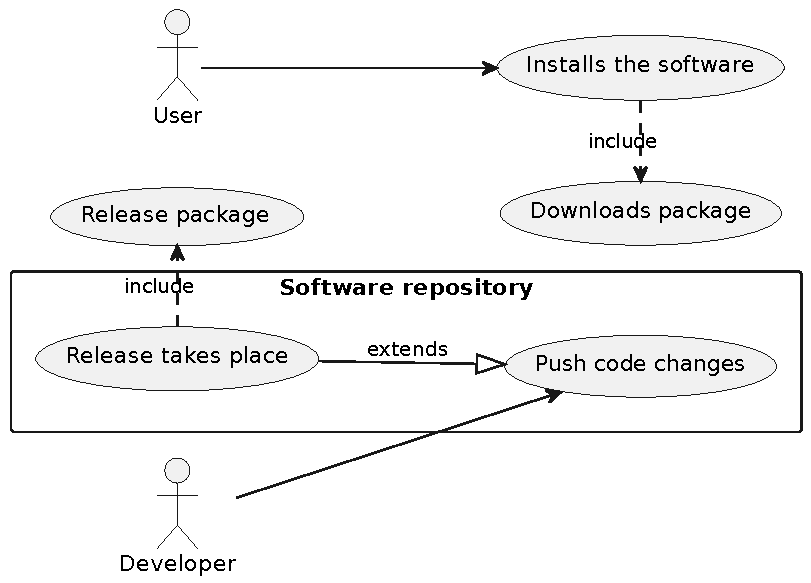
\includegraphics[width=.75\linewidth]{figures/use-case-diagram.pdf}
	\caption{Diagramma dei casi d'uso dallo sviluppatore all'utente}
	\label{fig:use-case-diagram}
	%https://alchemistsimulator.github.io/explanation/metamodel/
\end{figure}

L'obiettivo principale dell'elaborato è quindi quello di progettare un sistema di pacchettizzazione e distribuzione del software automatica all'interno di una pipeline di integrazione e distribuzione continua. I nuovi processi devono integrarsi all'interno dell'attuale pipeline di Alchemist, estendendo le funzionalità di assemblaggio di artefatti e rilascio del software. La distribuzione del pacchetto software deve avvenire per mezzo di repository pubblici diffusi, in modo da raggiungere il numero maggiore possibile di utenti; essa, inoltre, deve avvenire consistentemente nell'istante in cui una nuova versione di Alchemist viene rilasciata. La totalità dei processi integrati deve prevedere l'esecuzione di test all'interno del flusso, in modo da fornire un feedback immediato. Nella \Cref{fig:use-case-diagram} sono rappresentati gli scenari di utilizzo da parte degli utenti finali e gli sviluppatori di Alchemist. Lo sviluppatore introduce nuovo codice all'interno del repository del progetto, l'esecuzione della pipeline determina successivamente se il rilascio di una nuova versione è richiesto. L'effettiva distribuzione di una nuova versione include la generazione dei pacchetti software di installazione, i quali l'utente scarica per introdurre Alchemist nel proprio sistema.